%%%%%%%%%%%%%%%%%%%%%%%%%%%%%%%%%%%%%%%%%
% Beamer Presentation
% LaTeX Template
% Version 1.0 (10/11/12)
%
% This template has been downloaded from:
% http://www.LaTeXTemplates.com
%
% License:
% CC BY-NC-SA 3.0 (http://creativecommons.org/licenses/by-nc-sa/3.0/)
%
%%%%%%%%%%%%%%%%%%%%%%%%%%%%%%%%%%%%%%%%%

%----------------------------------------------------------------------------------------
%	PACKAGES AND THEMES
%----------------------------------------------------------------------------------------

\documentclass[compress]{beamer}

\mode<presentation> {
\setbeamertemplate{headline}{}
% The Beamer class comes with a number of default slide themes
% which change the colors and layouts of slides. Below this is a list
% of all the themes, uncomment each in turn to see what they look like.

%\usetheme{default}
% \usetheme{AnnArbor}
%\usetheme{Antibes}
%\usetheme{Bergen}
%\usetheme{Berkeley}
%\usetheme{Berlin}
%\usetheme{Boadilla}
%\usetheme{CambridgeUS}
%\usetheme{Copenhagen}
%\usetheme{Darmstadt}
%\usetheme{Dresden}
%\usetheme{Frankfurt}
%\usetheme{Goettingen}
%\usetheme{Hannover}
%\usetheme{Ilmenau}
%\usetheme{JuanLesPins}
%\usetheme{Luebeck}
%\usetheme{Madrid}
%\usetheme{Malmoe}
%\usetheme{Marburg}
%\usetheme{Montpellier}
%\usetheme{PaloAlto}q
%\usetheme{Pittsburgh}
%\usetheme{Rochester}
%\usetheme{Singapore}
%\usetheme{Szeged}
\usetheme{Warsaw}

% As well as themes, the Beamer class has a number of color themes
% for any slide theme. Uncomment each of these in turn to see how it
% changes the colors of your current slide theme.

%\usecolortheme{albatross}
%\usecolortheme{beaver}
%\usecolortheme{beetle}
%\usecolortheme{crane}
%\usecolortheme{dolphin}
%\usecolortheme{dove}
%\usecolortheme{fly}
%\usecolortheme{lily}
%\usecolortheme{orchid}
%\usecolortheme{rose}
%\usecolortheme{seagull}
%\usecolortheme{seahorse}
\usecolortheme{whale}
%\usecolortheme{wolverine}

%\setbeamertemplate{footline} % To remove the footer line in all slides uncomment this line
%\setbeamertemplate{footline}[page number] % To replace the footer line in all slides with a simple slide count uncomment this line

%\setbeamertemplate{navigation symbols}{} % To remove the navigation symbols from the bottom of all slides uncomment this line
}

\usepackage{graphicx} % Allows including images
\usepackage{booktabs} % Allows the use of \toprule, \midrule andxs                      % \bottomrule in tables
\usepackage{float}
\usepackage{caption}
\usepackage{subcaption}
\usepackage{listings} %syntax highlighting?
\usepackage{minted}
\usepackage{multicol} % table of contents
%\usepackage{subfigure}

%----------------------------------------------------------------------------------------
\graphicspath{ {./images/} }%	TITLE PAGE
%----------------------------------------------------------------------------------------
% \definecolor{mygreen}{cmyk}{0.82,0.11,1,0.25}
% \setbeamertemplate{blocks}[rounded][shadow=false]
% \addtobeamertemplate{block begin}{\pgfsetfillopacity{0.8}}{\pgfsetfillopacity{1}}
% \setbeamercolor{structure}{fg=mygreen}
\setbeamercolor*{block title example}{fg=black,
bg= gray!30}
\setbeamercolor*{block body example}{fg= black,
bg= gray!15}
\graphicspath{ {./images/}{./}{./timgs/}{./private/}}

\title[BioBots]{Biology was Robotics Before it was Cool.} % The short title appears at the bottom of every slide, the full title is only on the title page

\author{Katherine Scott} % Your name

\institute[@kscottz] % Your institution as it will appear on the bottom of every slide, may be shorthand to save space
{
Computer Vision Engineer
\medskip
\textit{katherine.a.scott@gmail.com}
\textit{http://www.kscottz.com}
}
\date{\today} % Date, can be changed to a custom date

\begin{document}

\begin{frame}
\titlepage % Print the title page as the first slide
\end{frame}

% \begin{frame}
%   \frametitle{Outline}
%   %\tableofcontents[pausesections,subsectionstyle=hide]
%   \tableofcontents[currentsection,sectionstyle=show,subsectionstyle=hide]
%   % You might wish to add the option [pausesections]
% \end{frame}

% \begin{frame}%{\contentsname}
% %\begin{multicols}{2}
% \frametitle{Overview} % Table of contents slide, comment this block out to remove it
% \tableofcontents % Throughout your presentation, if you choose to use \section{} and \subsection{} commands, these will automatically be printed on this slide as an overview of your presentation
% %\end{multicols}
% \end{frame}

%----------------------------------------------------------------------------------------
%	PRESENTATION SLIDES
%----------------------------------------------------------------------------------------
\section{Biology was Robotics Before It Was Cool}
\begin{frame}
  \frametitle{Biology was Robotics Before It Was Cool}
    \begin{figure}
     
\includegraphics[width=0.5\linewidth]{hipster.jpg}
   \end{figure}
   \begin{center}
   Nature had all of the good ideas first.
   \end{center}
\end{frame}
%----------------------------------------------------------------------------------------
\begin{frame}
  \frametitle{When I was a young}
  \begin{huge}
    When I was a young lady I didn't want to be a software engineer...
    \\~\\    
    I actually wanted to be a biomedical engineer.
    \\~\\
    Or some other kind of kick-ass scientist.
  \end{huge}
\end{frame}
%----------------------------------------------------------------------------------------
\begin{frame}
  \frametitle{My First Week at University of Michigan}
  \begin{figure}
    
\includegraphics[width=0.2\linewidth]{urop.jpg}
    \quad
    
\includegraphics[width=0.2\linewidth]{nsf.jpg}
  \end{figure}     
  \begin{itemize}
    \item Got up extra early. Looked through a big book. Picked the coolest one.
    \item \textbf{I had work study. UROP paid as well as waiting tables.} 
    \item Got to hang out in a lab. 
    \item \textit{By blind luck it was a robotics lab with a few women in it}.
  \end{itemize}
\end{frame}
%----------------------------------------------------------------------------------------
\begin{frame}
  \frametitle{DARPA Rules!}
  \begin{figure}
    \href{http://www.youtube.com/watch?v=_Ep-ehnXKvc}{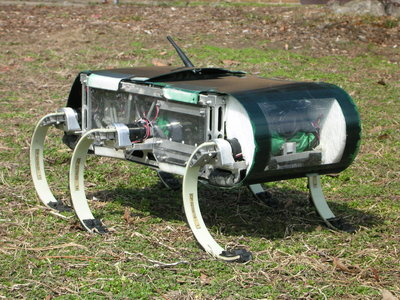
\includegraphics[width=0.4\linewidth]{rhex.jpg}}
    \quad
    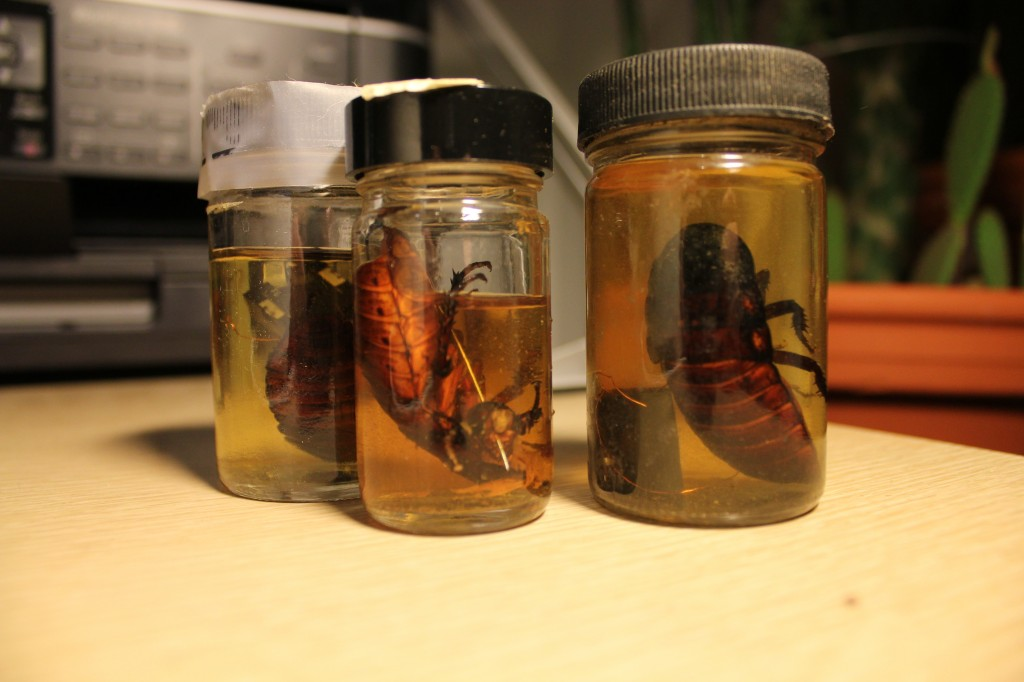
\includegraphics[width=0.4\linewidth]{bugs.jpg}
  \end{figure}     
  \begin{itemize}
    \item Lab was sponsored by the Defense Advanced Research Projects Agency (DARPA)
    \item Looking at how cockroaches moved. Can we replicate it?
    \item Instead of making robots that moved like roaches can we control roaches like robots?
  \end{itemize}
\end{frame}
%----------------------------------------------------------------------------------------
\begin{frame}
  \frametitle{Turns out there are no unsolved problems in robotics.}
  \begin{figure}
    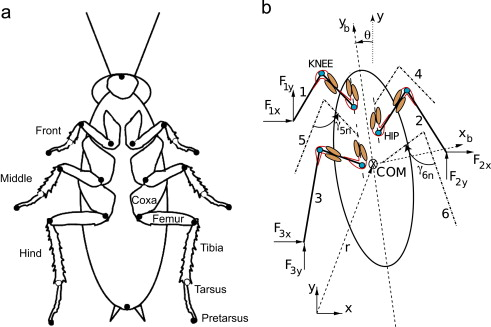
\includegraphics[width=0.6\linewidth]{roach.jpg}
  \end{figure}     
  \begin{itemize}
    \item Mother nature has got this stuff solved. 
    \item The sensors, actuators, and controllers on this bug are perfect.
    \item We just need to take it apart and figure out how it works. 
  \end{itemize}
\end{frame}
%----------------------------------------------------------------------------------------
\begin{frame}
  \frametitle{}
  \begin{figure}
    
\includegraphics[width=0.6\linewidth]{byb.png}
  \end{figure}     
  Some of my old lab mates wanted to educate students on neuroscience. They commericalized some of the technology so students could learn from it. They kindly donated materials for today!
\end{frame}
%----------------------------------------------------------------------------------------

\begin{frame}
  \frametitle{What about the inverse problem? Can we make roaches robots?}
  \begin{figure}
    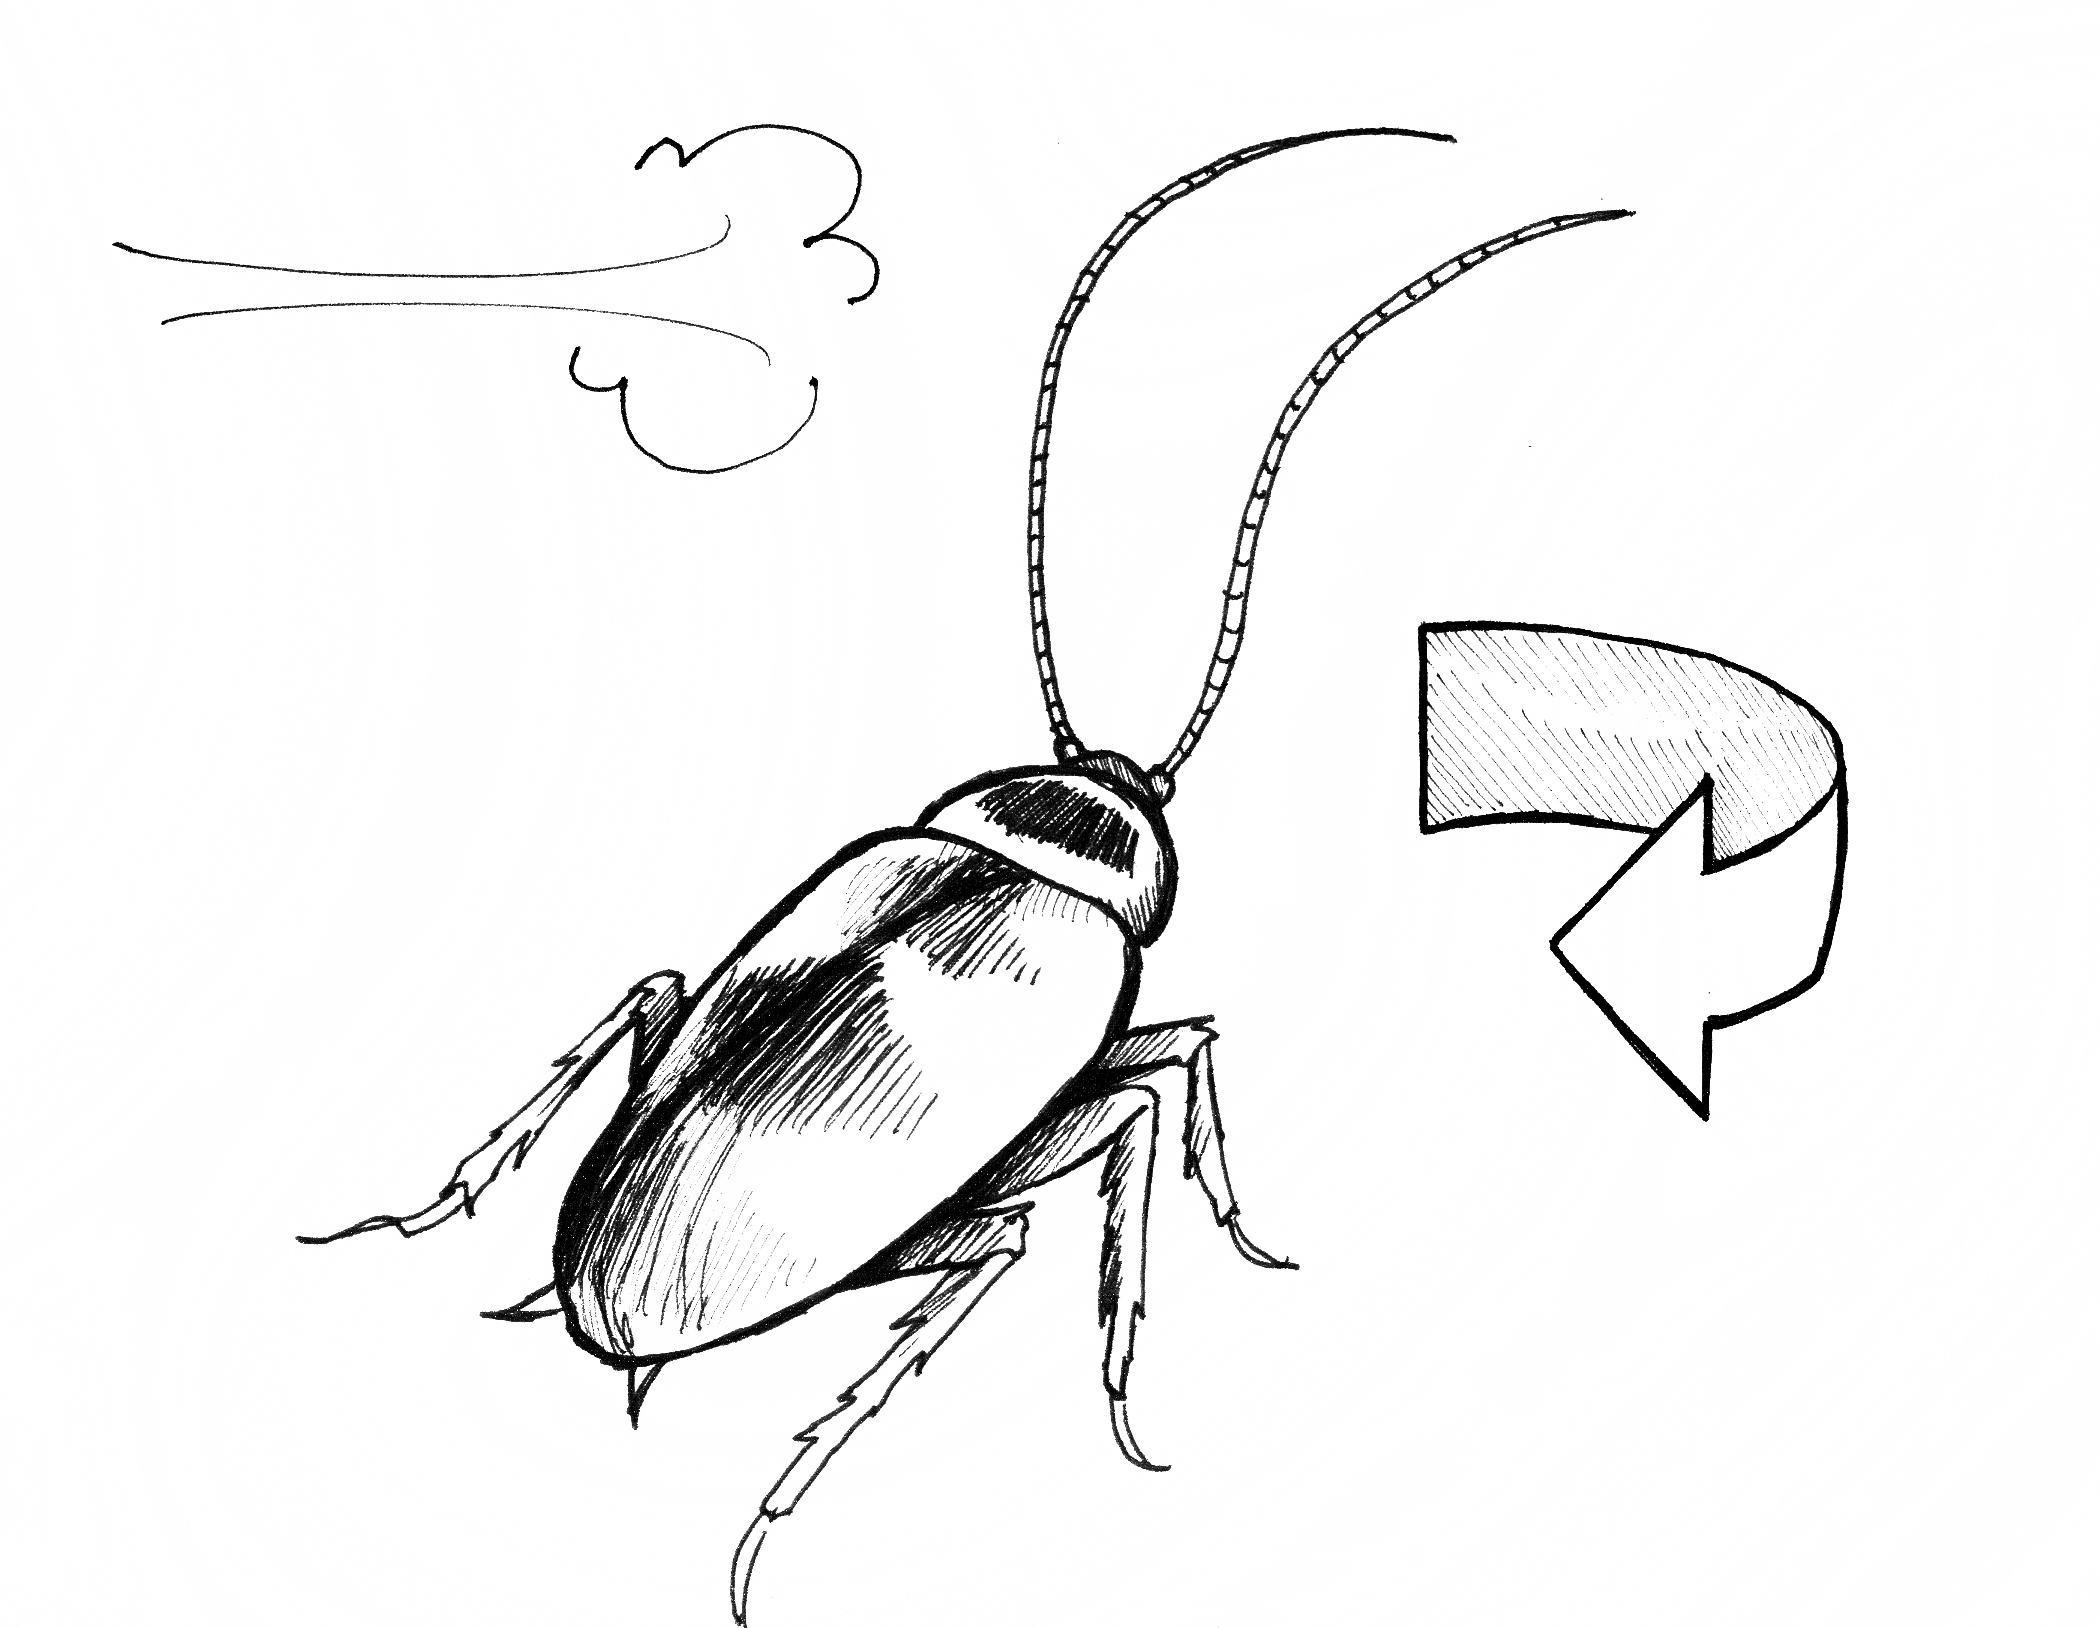
\includegraphics[width=0.8\linewidth]{wind.jpg}
  \end{figure}     
\end{frame}

%----------------------------------------------------------------------------------------
\begin{frame}
  \frametitle{Remember your sensors...}
  \begin{figure}
    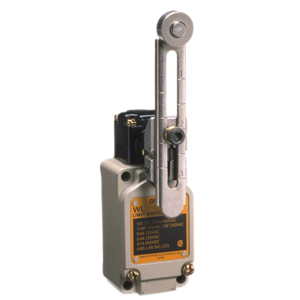
\includegraphics[width=0.4\linewidth]{limit.jpg}
  \end{figure}     
  \begin{center}
    Limit switch.... 
  \end{center}
\end{frame}
%----------------------------------------------------------------------------------------
\begin{frame}
  \frametitle{Can we hack into the roaches' sensors?}
  \begin{figure}
    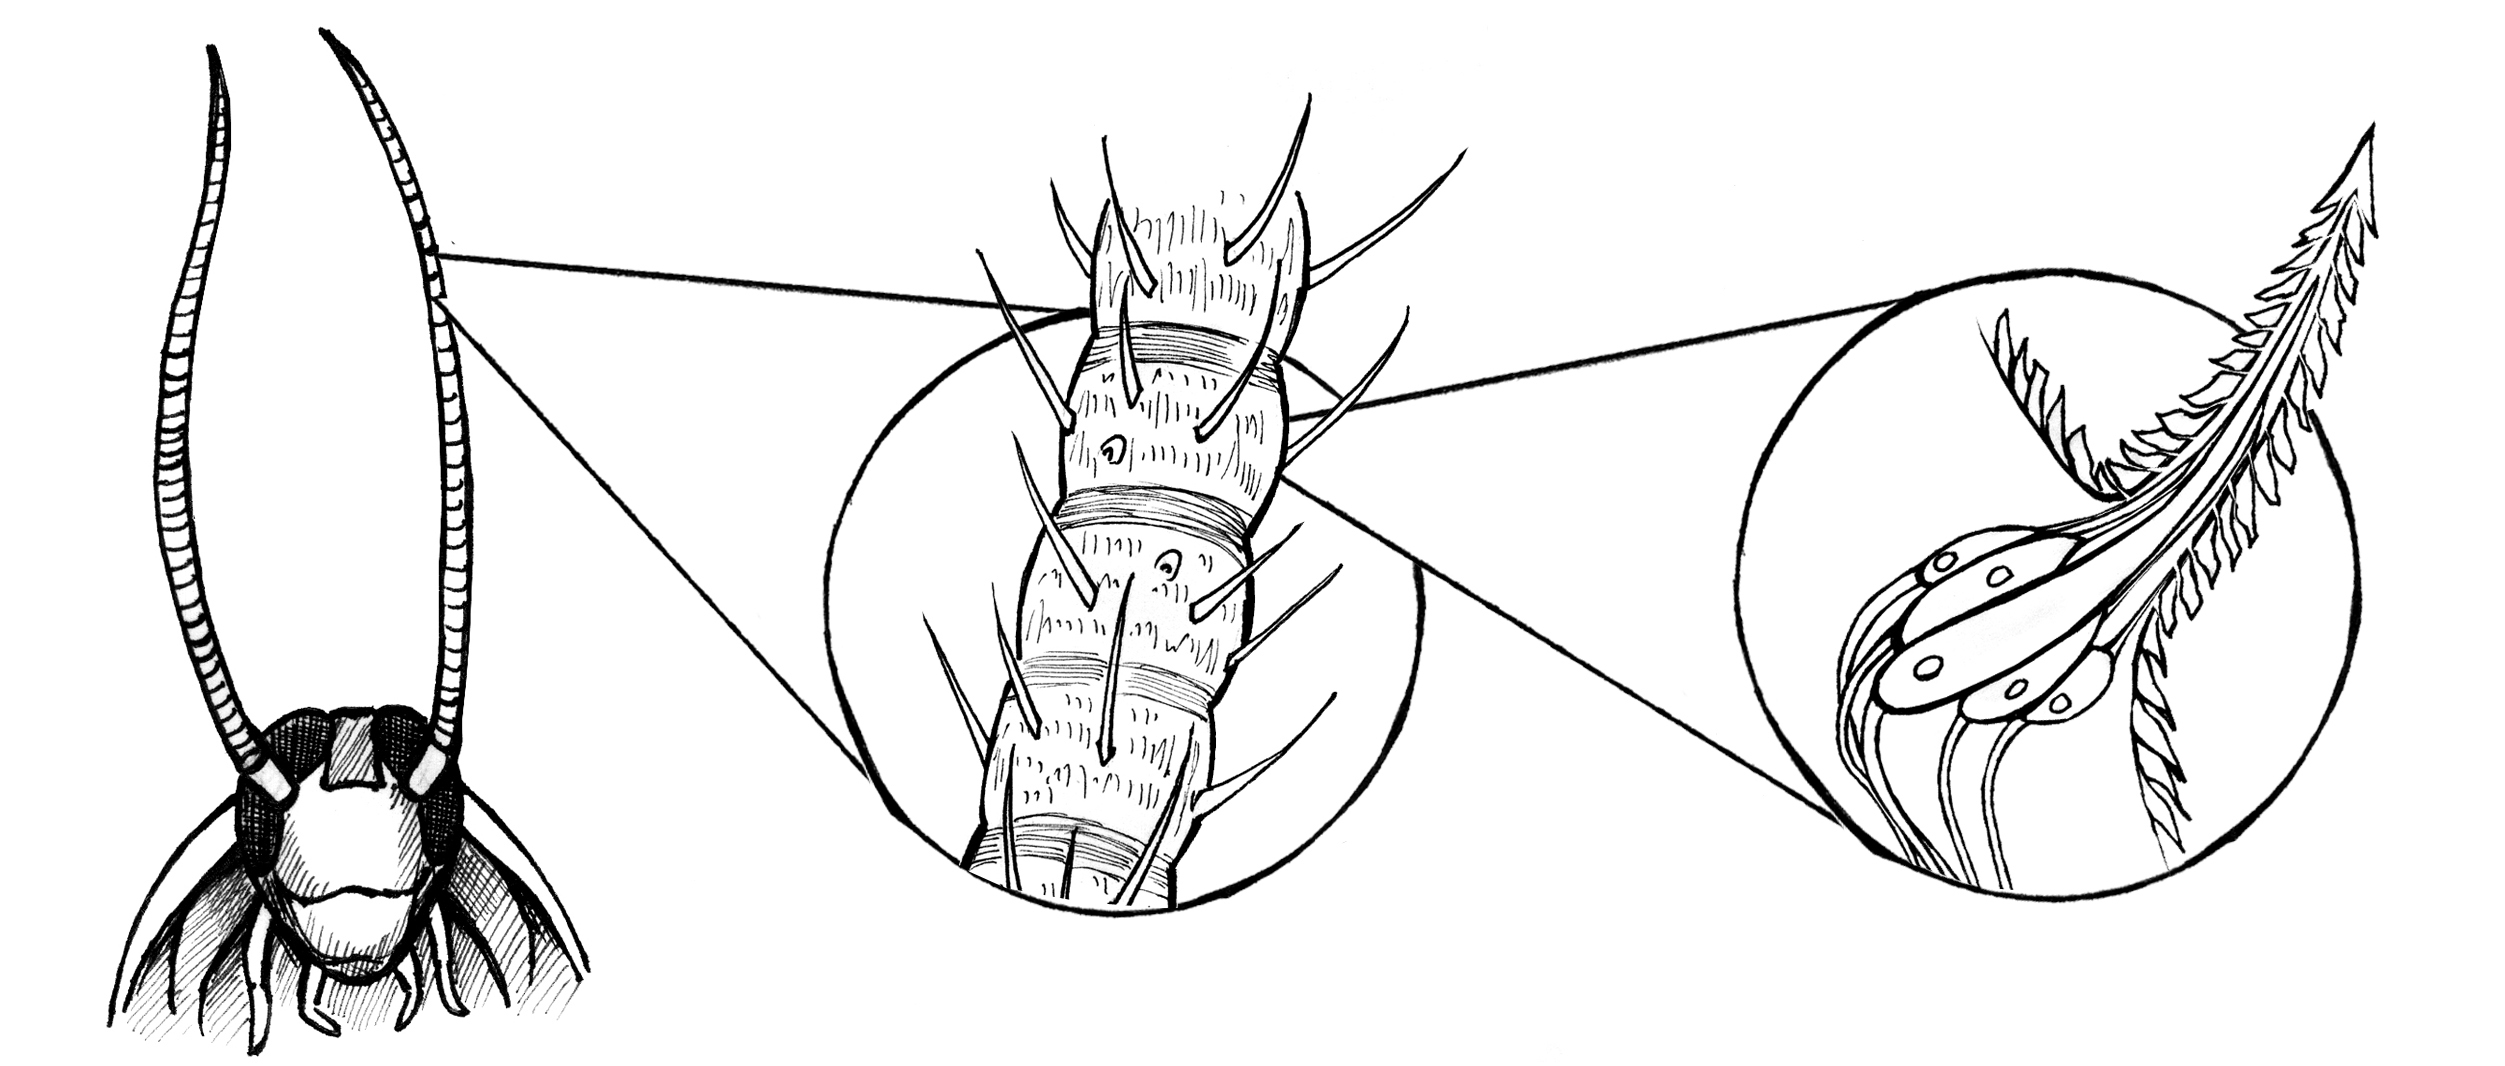
\includegraphics[width=0.8\linewidth]{combo2.jpg}
  \end{figure}     
\end{frame}
%----------------------------------------------------------------------------------------
\begin{frame}
  \frametitle{How does a roach work?}
  \begin{itemize}
    \item +/-3V Signal
    \item Biphasic Square Wave
    \item Roughly 10-100Hz 
    \item Emulates the signal the neurons would generate. 
    \item Don't worry, the roach will be just fine, we'll leave him a lot of sensor.
    \end{itemize}
\end{frame}
%----------------------------------------------------------------------------------------
\begin{frame}
  \frametitle{So what is going on here?} 
  \begin{figure}
    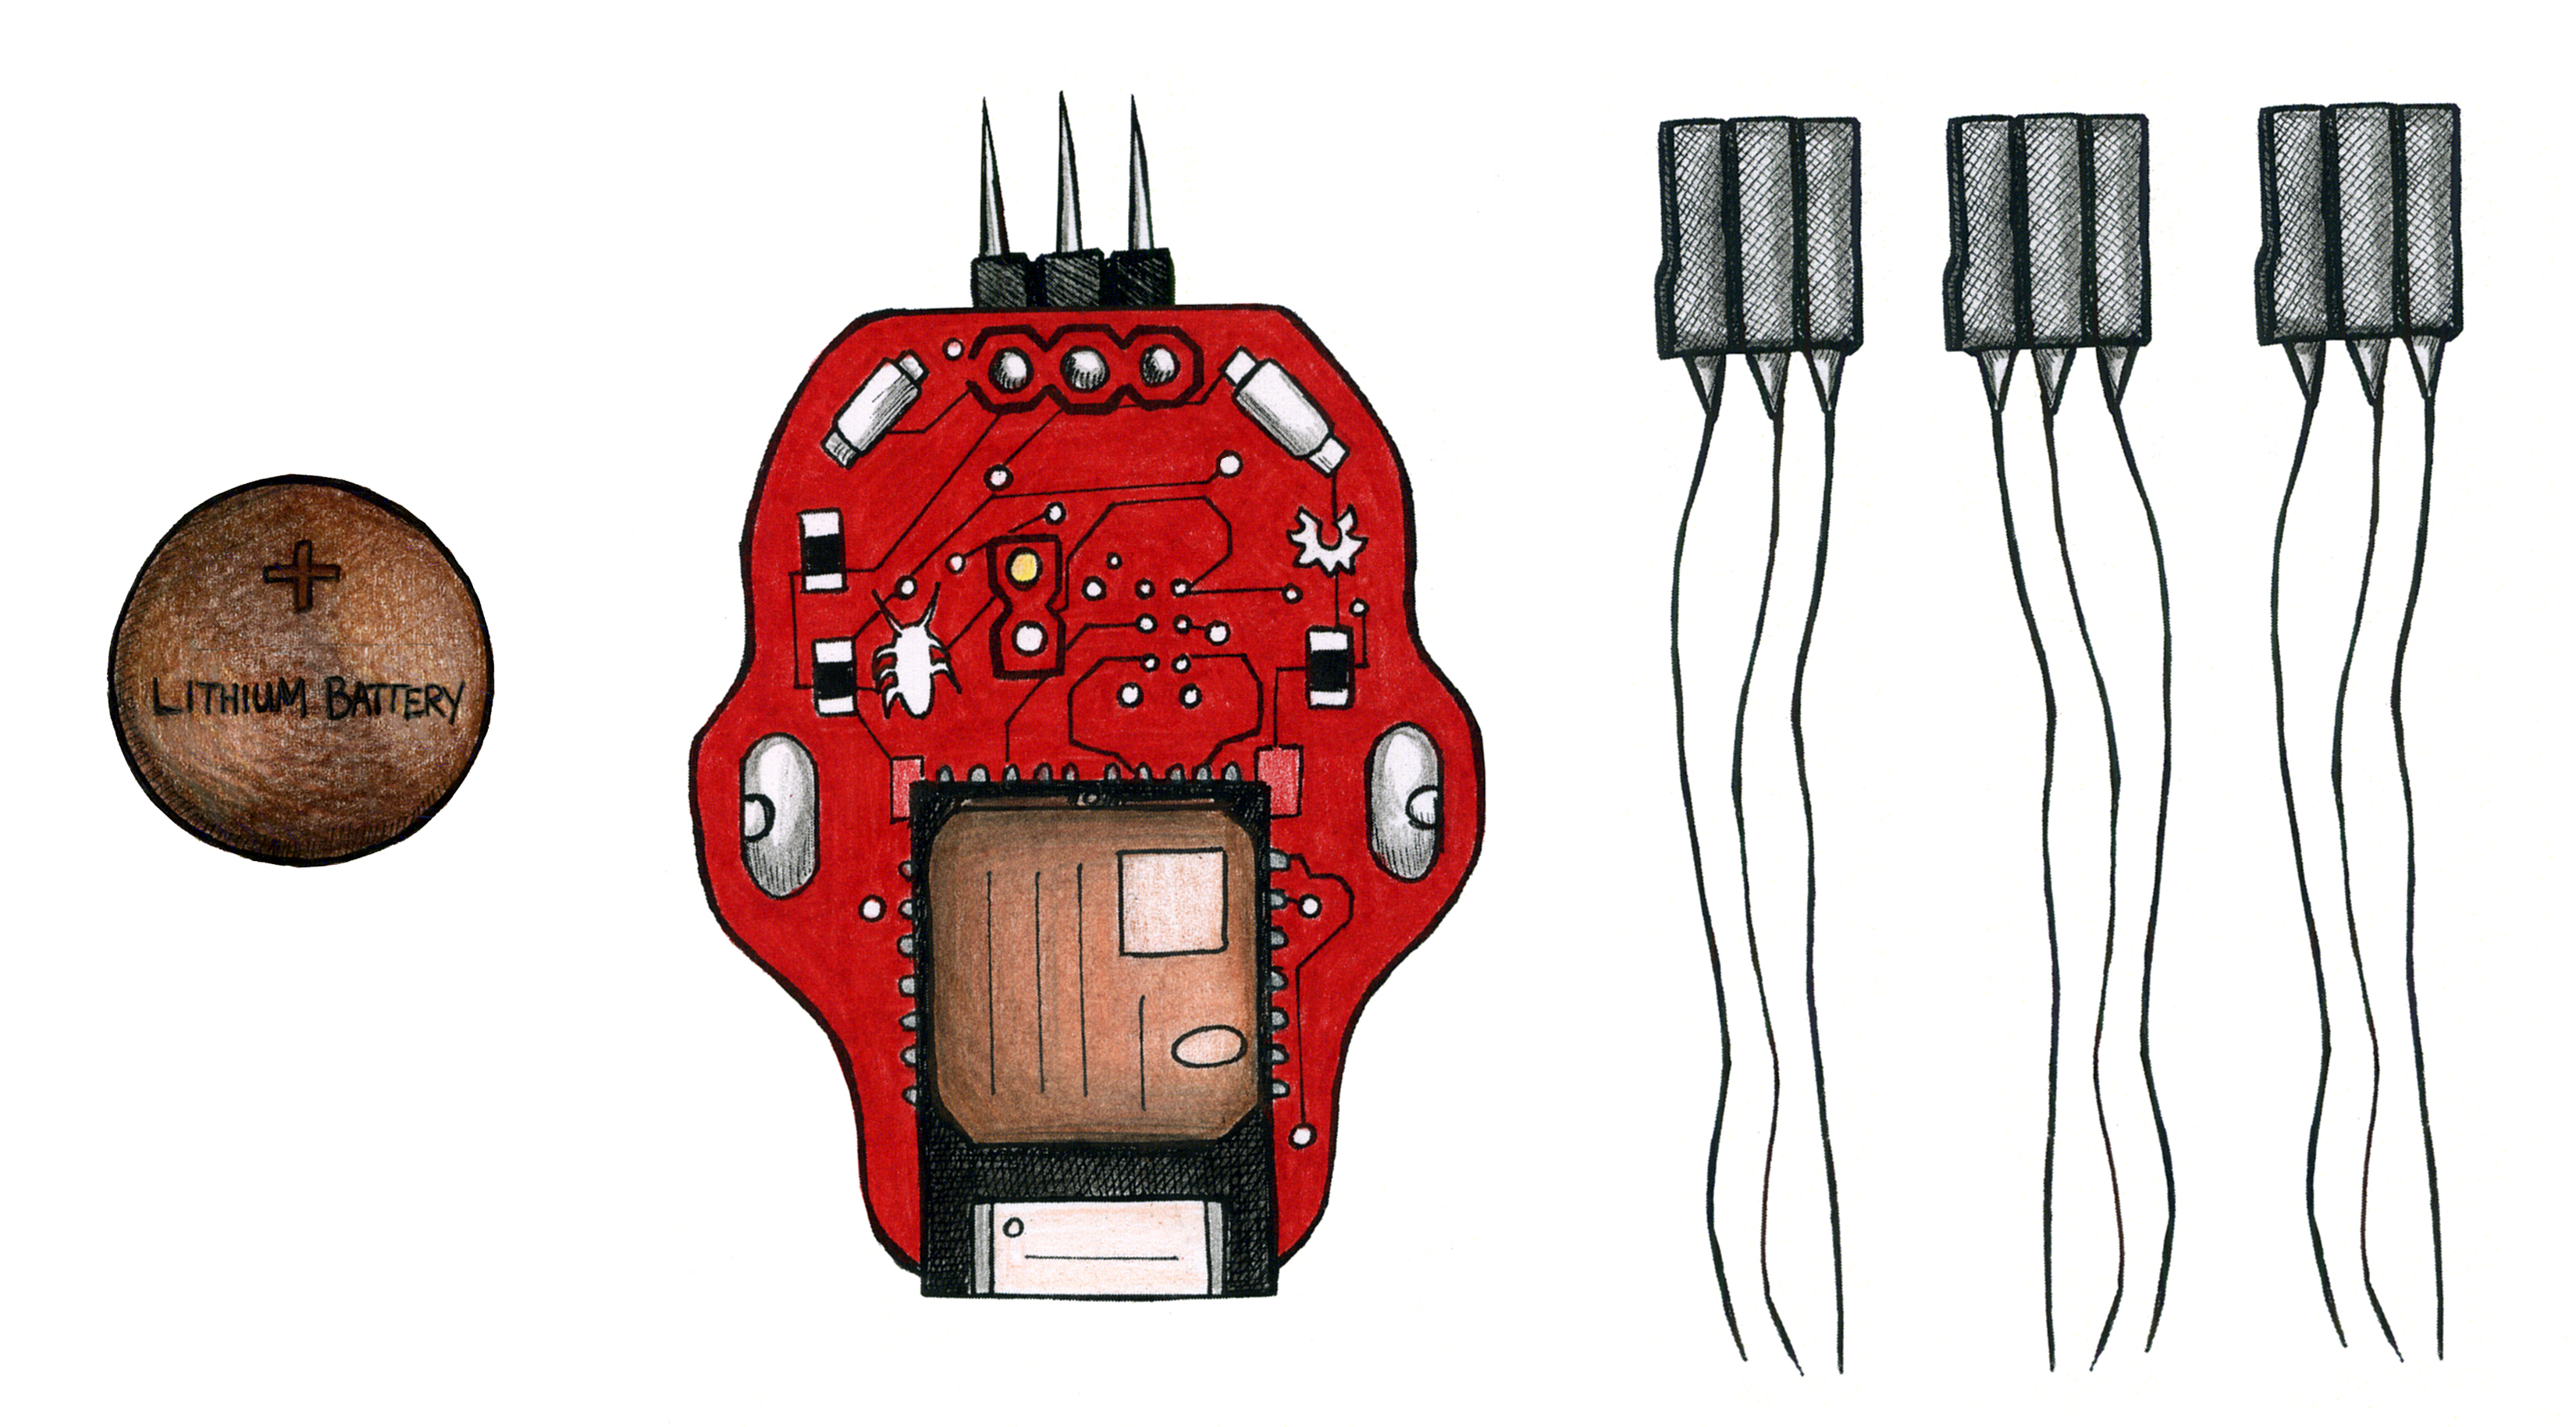
\includegraphics[width=0.7\linewidth]{box1.jpg}
  \end{figure}     
  \begin{itemize}
    \item Control signals sent from phone via bluetooth.
    \item On the board bluetooth cpu gets the message, and generates a waveform.
    \item We then amplify it a bit and send it to the roach via leads. 
    \item Roach says, gee, feels like something is there. 
  \end{itemize}
\end{frame}
%----------------------------------------------------------------------------------------
\begin{frame}
  \huge{So should we give it a try?}
\end{frame}
%----------------------------------------------------------------------------------------
\begin{frame}
  \frametitle{Could we take this to the next level?}
  \begin{figure}
    \href{http://www.youtube.com/watch?v=R-IzkGA9hTc}{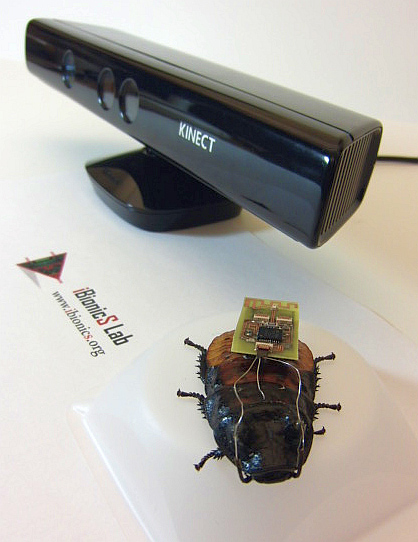
\includegraphics[width=0.5\linewidth]{autopilot.jpg}}
  \end{figure}     
\end{frame}
%----------------------------------------------------------------------------------------
\begin{frame}
  \frametitle{What are the parts to getting this done?}
   \textit{\textbf{DO NOT PANIC.} Break the problem down to little chunks and solve each chunk.}
  \begin{itemize}
    \item Find a bluetooth library to ``talk'' to the roach backpack.
    \item Find a library that can get images from the kinect.
    \item \href{http://www.simplecv.org}{Write some code to get the roach position / orientation.}
    \item Write some code to find the line.
    \item Write some code that figures out the difference between the roach and the line.
    \item Figure out a way to relate that difference to stimulation.
  \end{itemize}
\end{frame}
%----------------------------------------------------------------------------------------
\begin{frame}
  \frametitle{Roaches are just the tip of the iceberg...}
  \begin{figure}
    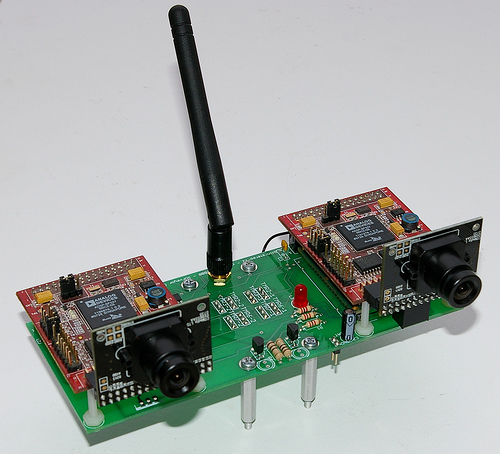
\includegraphics[width=0.35\linewidth]{stereo.jpg}
    \quad
    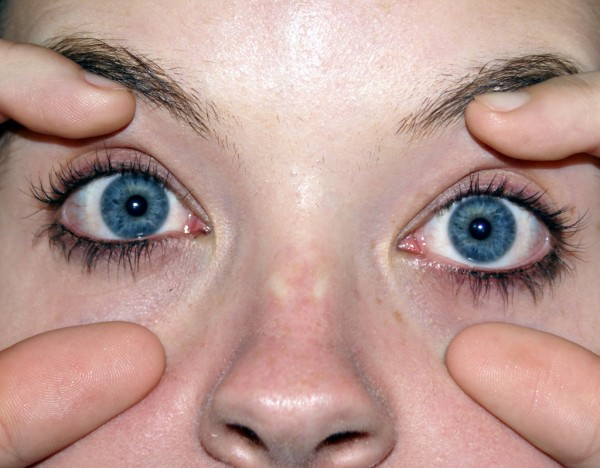
\includegraphics[width=0.35\linewidth]{eyes.jpg}
  \end{figure}     
  Stereo vision is something we use everyday, why not robots?
\end{frame}
%----------------------------------------------------------------------------------------
\begin{frame}
  \frametitle{Roaches are just the tip of the iceberg...}
  \begin{figure}
    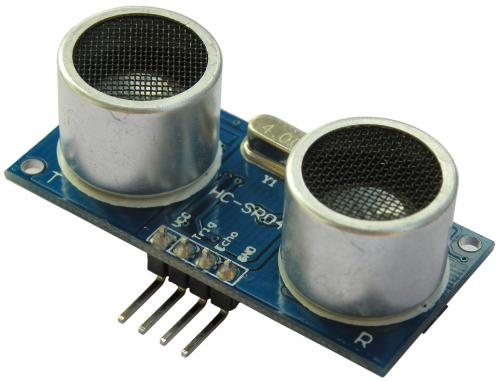
\includegraphics[width=0.35\linewidth]{sonar.jpg}
    \quad
    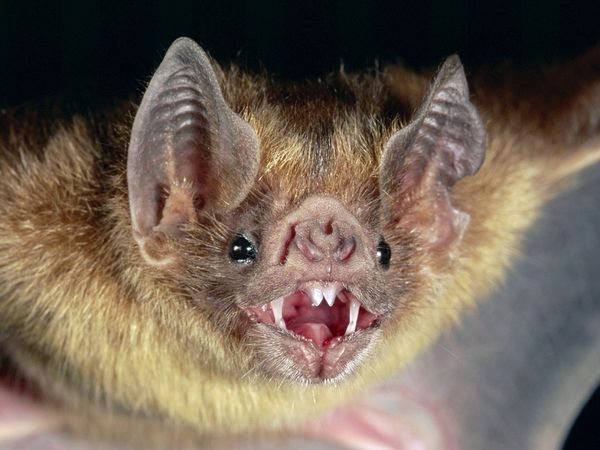
\includegraphics[width=0.35\linewidth]{bat.jpg}
  \end{figure}     
  Bats get around with sonar, why not robots?
\end{frame}

%----------------------------------------------------------------------------------------
\begin{frame}
  \frametitle{Roaches are just the tip of the iceberg...}
  \begin{figure}
    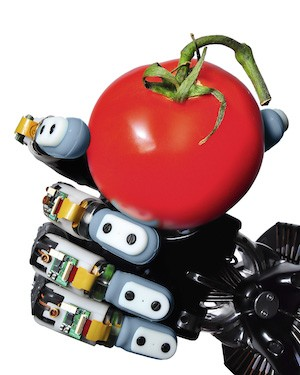
\includegraphics[width=0.35\linewidth]{robohand.jpg}
    \quad
    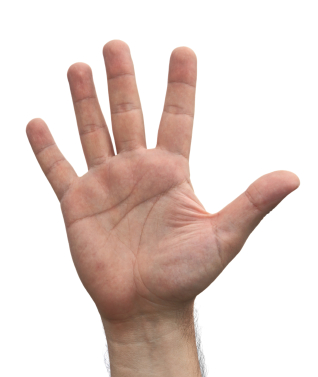
\includegraphics[width=0.35\linewidth]{hand.jpg}
  \end{figure}     
 We can figure out stuff with our hands? Why not robots?
\end{frame}
%----------------------------------------------------------------------------------------
\begin{frame}
  \frametitle{The best part about robotics.}
  \begin{figure}
    
\includegraphics[width=0.5\linewidth]{chained.jpg}
  \end{figure}     
  You'll never be chained to a desk. You'll be working with every engineering discipline, biologists, psychologists, and designers. It really is a true interdisciplinary field. 
\end{frame}
%----------------------------------------------------------------------------------------
%----------------------------------------------------------------------------------------
\begin{frame}
  \frametitle{GO BUILD ROBOTS!}
  Here are a few resources to get you started!
  \begin{itemize}
    \item \href{http://www.backyardbrains.com}{Back Yard Brains}
    \item \href{http://store.iheartengineering.com/robots/turtlebot.html}{I Heart Robotics}
    \item \href{http://www.usfirst.org/roboticsprograms/frc}{FIRST Robotics Competition}
    \item \href{http://www.ros.org/wiki/}{Robot Operating System (ROS)}
    \item \href{http://nodebots.io/}{Nodebots!}
    \item \href{https://github.com/hugs/tapsterbot}{Build a Tapsterbot}
    \item \href{http://hackerspaces.org/wiki/List_of_Hacker_Spaces}{GO VISIT A HACKER SPACE.}
  \end{itemize}
\end{frame}
%----------------------------------------------------------------------------------------


\end{document} 
